\documentclass[runningheads,a4paper]{llncs}

\usepackage{amssymb}
\setcounter{secnumdepth}{5}
\setcounter{tocdepth}{3}
\usepackage{graphicx}
\usepackage{floatrow}
\usepackage{url}
\newcommand{\keywords}[1]{\par\addvspace\baselineskip
\noindent\keywordname\enspace\ignorespaces#1}

\begin{document}

\mainmatter 

\title{RoboCup SPL 2015 Champion Team Paper}
\titlerunning{SPL 2015 Champion Team Paper}

\author{
Brad Hall
\and Sean Harris
\and Bernhard Hengst
\and Roger Liu
\and Kenneth Ng
\and Maurice Pagnucco
\and Luke Pearson
\and Claude Sammut
\and Peter Schmidt
}
\authorrunning{Hall, et. al.}

\institute{
School of Computer Science and Engineering\\
University of New South Wales\\
Sydney 2052 Australia\\
\url{http://www.cse.unsw.edu.au}}

\maketitle

\begin{abstract}
The Robocup Standard Platform League competition is a highly competitive league, with very little separating the top teams. Winning the competition in consecutive years is particularly challenging as other teams look to counter the tactics and game play of the previous champions. As the reigning champions from 2014, team UNSW Australia was able to overcome this challenge and win the competition for a second consecutive year. Although this success is not only related to developments from this year, this paper focuses on the new innovations and development by team UNSW Australia for the 2015 Robocup Competition. These innovations include white goal detection, whistle detection, foot detection and avoidance, improved path planning and new odometry.
\end{abstract}





\section{Introduction}
Team \emph{UNSW Australia}, formerly known as \emph{rUNSWift}, has been competing in the Standard Platform League (SPL) since 1999. We were world champions 3 times in the years 2000-2003, but were unable to regain that title until 2014, when we won the competition for the first time in eleven years. In 2015 we successfully defended our title, to become back-to-back champions for the first time since 2000-2001.

The competition in 2015 introduced new challenges for the teams. The goal posts changed from being a distinct yellow colour, to being a standard white, making them significantly less unique and harder to detect. The finals matches were started by a human referee blowing a whistle, rather than a wifi packet. Teams were also permitted to wear unique jersey colours, instead of the previous cyan and magenta standard colours.

In addition to this, the 2015 team also faced UNSW specific challenges. After a successful 2014 campaign involving a large team of alumni and current students, we had an exceptionally high turnover rate. This lead to almost an entirely new team, who had little to no experience with the code base before 2015. This also resulted in a smaller team, and thus limited the scope of new innovations in 2015.

The 2015 UNSW Australia team members are Sean Harris, Roger Liu, Kenneth Ng, Luke Pearson, Peter Schmidt and faculty members Brad Hall, Bernhard Hengst, Maurice Pagnucco and Claude Sammut, many of whom are shown in Figure \ref{teamphoto}.

\begin{figure}[h]
\centering
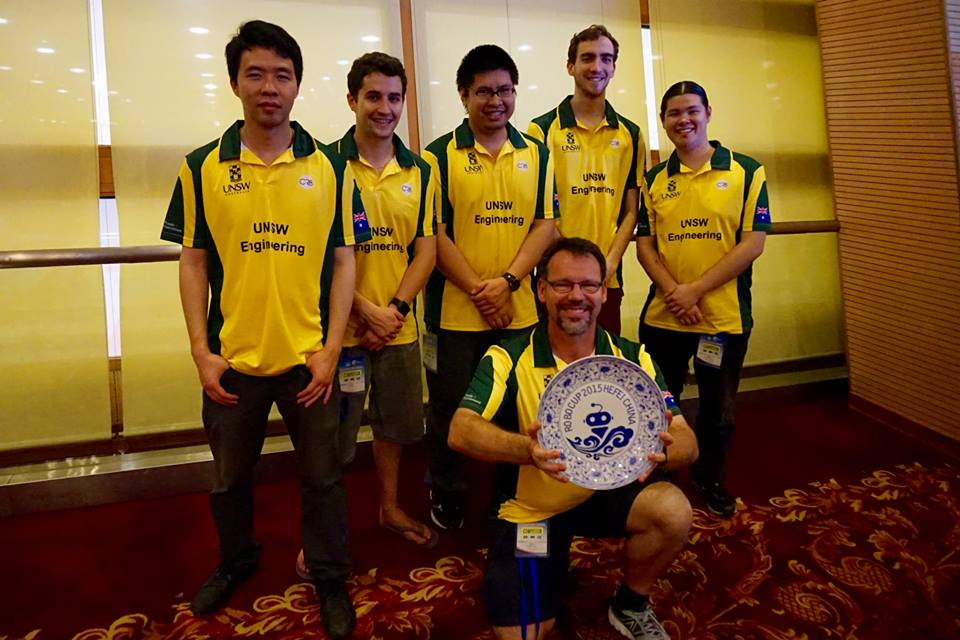
\includegraphics[width=0.8\textwidth]{Figures/TeamPhoto.jpg}
\caption{A subset of the 2015 team. From left to right: Roger Liu, Sean Harris, Kenneth Ng, Luke Pearson, Peter Schmidt. Kneeling: Brad Hall}
\label{teamphoto}
\end{figure}

The success of our campaign cannot be attributed to a single contribution, nor only this year's improvements. Our success in 2015 was a combination of previous success \cite{2014runswift}, strong team culture and continued innovation in all areas of robot soccer. This paper outlines the innovations of the 2015 team, including new goal detection, whistle detection, foot detection and avoidance, path planning and odometry.


\section{Team Organisation and Development Methodologies}
Consistent team organisation and routines have played a significant role in the success of the rUNSWift team in recent years. Despite a significant turnover of students moving from 2014 to 2015, the team maintained the regular meeting and testing routines used in 2014.

The team would meet once a week, utilising Google Hangouts when geography made physical meetings challenging. At these meetings each team member would outline their progress over the previous week, ask questions about topics that were challenging and set goals for the next week. This process made all team members accountable for their actions (or lack thereof) over the past week and ensured everyone remained focused. It also allowed team members to ask for assistance on difficulties they had experienced and fostered a culture of support for other team members.

The team also maintained regular testing schedules. The simplest of these is a  `striker test', where a single robot and the ball are placed in set positions around the field, and the time taken to score a goal is measured. This tests the integration of all our modules and improvements over the past week to ensure that changes are actually improving our overall soccer play. We also ran regular practice drills and matches involves multiple robots to test team play, positioning and obstacle avoidance.

\section{Whistle Detection}

In 2015 the SPL Rules changed to have all finals games start by a human referee's whistle sound. In the past a wifi packet was used to signal the kick off. The wifi packet was not removed in 2015, but instead was delayed 15 seconds, providing a significant advantage to teams who were able to successfully and reliably detect the whistle. We identified two key problems to solve in successfully implementing a whistle detector. The first was to detect true positive whistles reliably, and the second to avoid false positives from other noises or far away whistles.

To assist with this, the free open source software tool Audacity was used. Figure \ref{figWhistleAnalysis} contains an example Audacity project. Conceptually from Figure \ref{figWhistleAnalysis} our whistle detection algorithm looks for a white or red rectangle in the 2000-4000 Hz range lasting for at least 250 ms.

\begin{figure}[h]
\centering
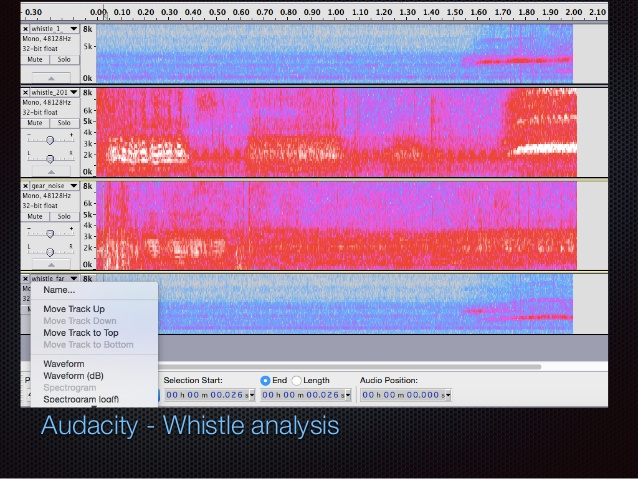
\includegraphics[width=0.8\textwidth]{Figures/figWhistleAnalysis}
\caption{
   An Audacity Project with tracks switched to spectrogram view.
   From top to bottom:
   A quiet whistle in the UNSW Robocup lab,
   a loud whistle at Hefei competition,
   a gear noise false positive and
   a far away whistle in the lab.
}
\label{figWhistleAnalysis}
\end{figure}

To detect a whistle signal, the algorithm integrates 3 main ideas on the NumPy Fast Fourier Transform of raw audio data, henceforth referred to as the spectrum. Firstly, we adaptively grow background noise zones by discarding 200Hz sections from the low and high end of the spectrum, leaving a smaller signal to focus on. Secondly, we only count the spectrum if the remaining signal is statistically quiet relative to the whole spectrum. Thirdly, we only count the spectrum if it is statistically quiet compared to the spectra recorded over the previous second.

Our whistle detection code runs in a separate Python process, and is fairly resource intensive. It consumes approximately $30-40\%$ of CPU time on the Nao, which is far too expensive to run at all times. Thus we only trigger the whistle detection once the game state switches to `Ready', which means we are expecting a whistle shortly. Once the game begins we then turn off the whistle detection until the next time it is required. Figure \ref{figWhistleDataFlow} shows the usage and development cycle for the whistle detection system. All previously recorded whistle sounds are downloaded after a game and the regression test is updated to include the new samples.

\begin{figure}
\centering
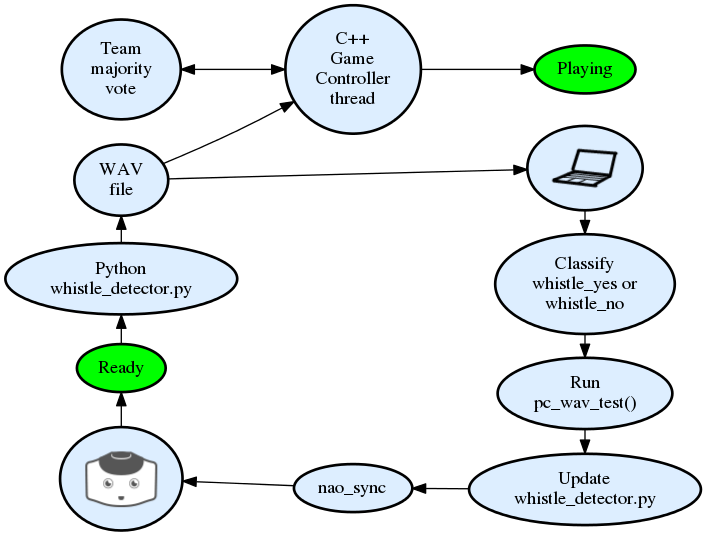
\includegraphics[width=0.8\textwidth]{Figures/figWhistleDataFlow}
\caption{Whistles: Overview of the development and data flows through the Nao. Green circles indicate a game state change. Note that the laptop subsystem is external and occurs after each game.}
\label{figWhistleDataFlow}
\end{figure}

To improve the reliability of the overall team system, the final decision for whether or not the game has begun is made by a team vote. Once a majority of players agree that the whistle has been blown, the whole team will start playing, regardless of what they voted. This system allowed us to handle infrequent false positives and true negatives by repeating the experiment across all 5 robots and taking the majority decision.

At the competition, our team was perfect at detecting whistles. The team never false started before the whistle had been blown and also never failed to start on a correct whistle. This was despite numerous nearby whistles during games that often fooled human spectators. We were the only team to have a perfect record in detecting the whistle at the 2015 competition.

\section{Foot detection and Avoidance}

Foot detection and avoidance was introduced into the 2015 rUNSWift codebase with the goal of reducing the total number of falls that occur as a result of stepping on another robot's foot. 

Foot detection works by scanning image for strong edge points. Following this it removes straight lines from the image with RANSAC. It then performs a custom point filtering algorithm which aims to remove points that are unlikely to be part of a robot. The main assumption here is that any vertical rectangular region of non-green coloured pixels is likely to be a robot. Thus we identify any points that have a substantial run of non-green pixels above them and mark them as candidate points. Then any points that aren't candidate points, nor are near candidate points, are removed. This results in points belonging to only field lines being removed, whilst maintaining points on the feet of nearby robots. Following this only the bottom points in the set are kept, i.e. only one point per $x$ location which is minimal in $y$. This works on the assumption that the foot should be at the bottom of the image. A successful detection is shown in Figure \ref{figFeet}.

\begin{figure}[h]
\centering
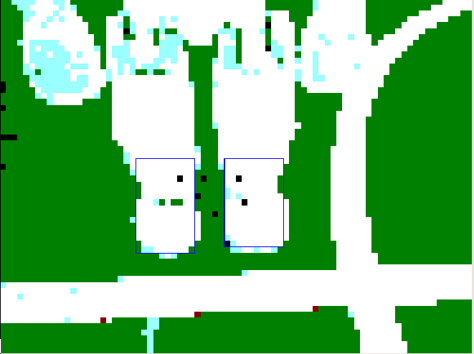
\includegraphics[scale=0.7]{Figures/figFeet}
\caption{
   The colour saliency provided from offnao (our offline debugger) with the feet bounding boxes shown in blue. The image also includes a difficult case of field line intersection which has not been classified as feet.
}
\label{figFeet}
\end{figure}

Finally the points are bucketed and the midpoint of the bucket is calculated using the following formula:

\begin{equation}
Midpoint = (\frac{\sum_{i=0}^{|B|} B_{xi}}{|B|}, \frac{\sum_{i=0}^{|B|} B_{yi}}{|B|}  )
\end{equation}

Following the bucketing, a region is grown using a breadth first search (BFS) that is bounded by a set of rules. A bounding box is created by taking the minimum $x$, $y$, and maximum $x$, $y$ values visited during the BFS.

The bounding boxes are then passed onto the walk module and used to clip the walk parameters as required. A step is defined with three parameters, $forward$, $left$ and $turn$ as shown in Figure \ref{figWalkParam}. $Forward$ specifies the intended $x$ location of the foot after the step in coordinates relative to the robot, $left$ specifies the intended $y$ location of the foot, and $turn$ specifies the rotation of the foot during the step. These parameters are adjusted to be within the physical capabilities of the robot. The parameters are then tested to see whether they fall within a bounding box, which represents the opponent's feet. This is done by intersecting a circle, which represents the toe of our robot, with the set of opponent feet. If the toe lands in any of the boxes the parameters are scaled down. This process is repeated until no intersection occurs.

\begin{figure}
\centering
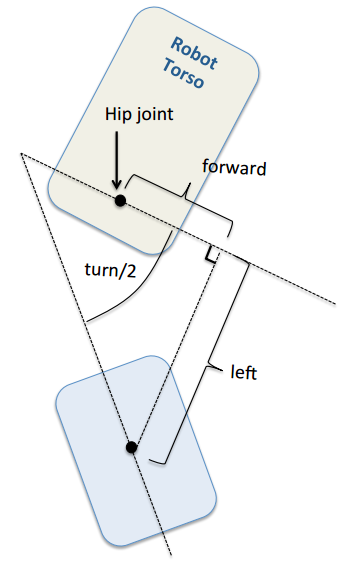
\includegraphics[scale=0.3]{Figures/figWalkParam}
\caption{
   The walk parameters and the resulting location of the foot.
}
\label{figWalkParam}
\end{figure}

Foot detection and avoidance proved to be substantially better than having no such system in place. We measured this by examining ``danger instances'', which represent instances where it was possible to step on, and detect, the opponent's toes. Our 2014 matches had 1 fall every 4.7 danger instances, and our 2015 matches had 1 every 10.1 danger instances. In 2014 there was a 21.2\% chance of stepping on a toe in every danger instance, this percentage is reduced to 9.8\% with foot detection and avoidance.

\section{Motion}
Competitive bipedal soccer playing robots need to move fast and react quickly to changes in direction while staying upright. An overview of the UNSW motion module is provided in an internal technical report \cite{hengst2014walk}. This report describes our approach to reactive omni-directional locomotion for the Nao robot as used in the RoboCup Standard Platform League competitions in 2014 and 2015.

\begin{figure} [ht]
\centering
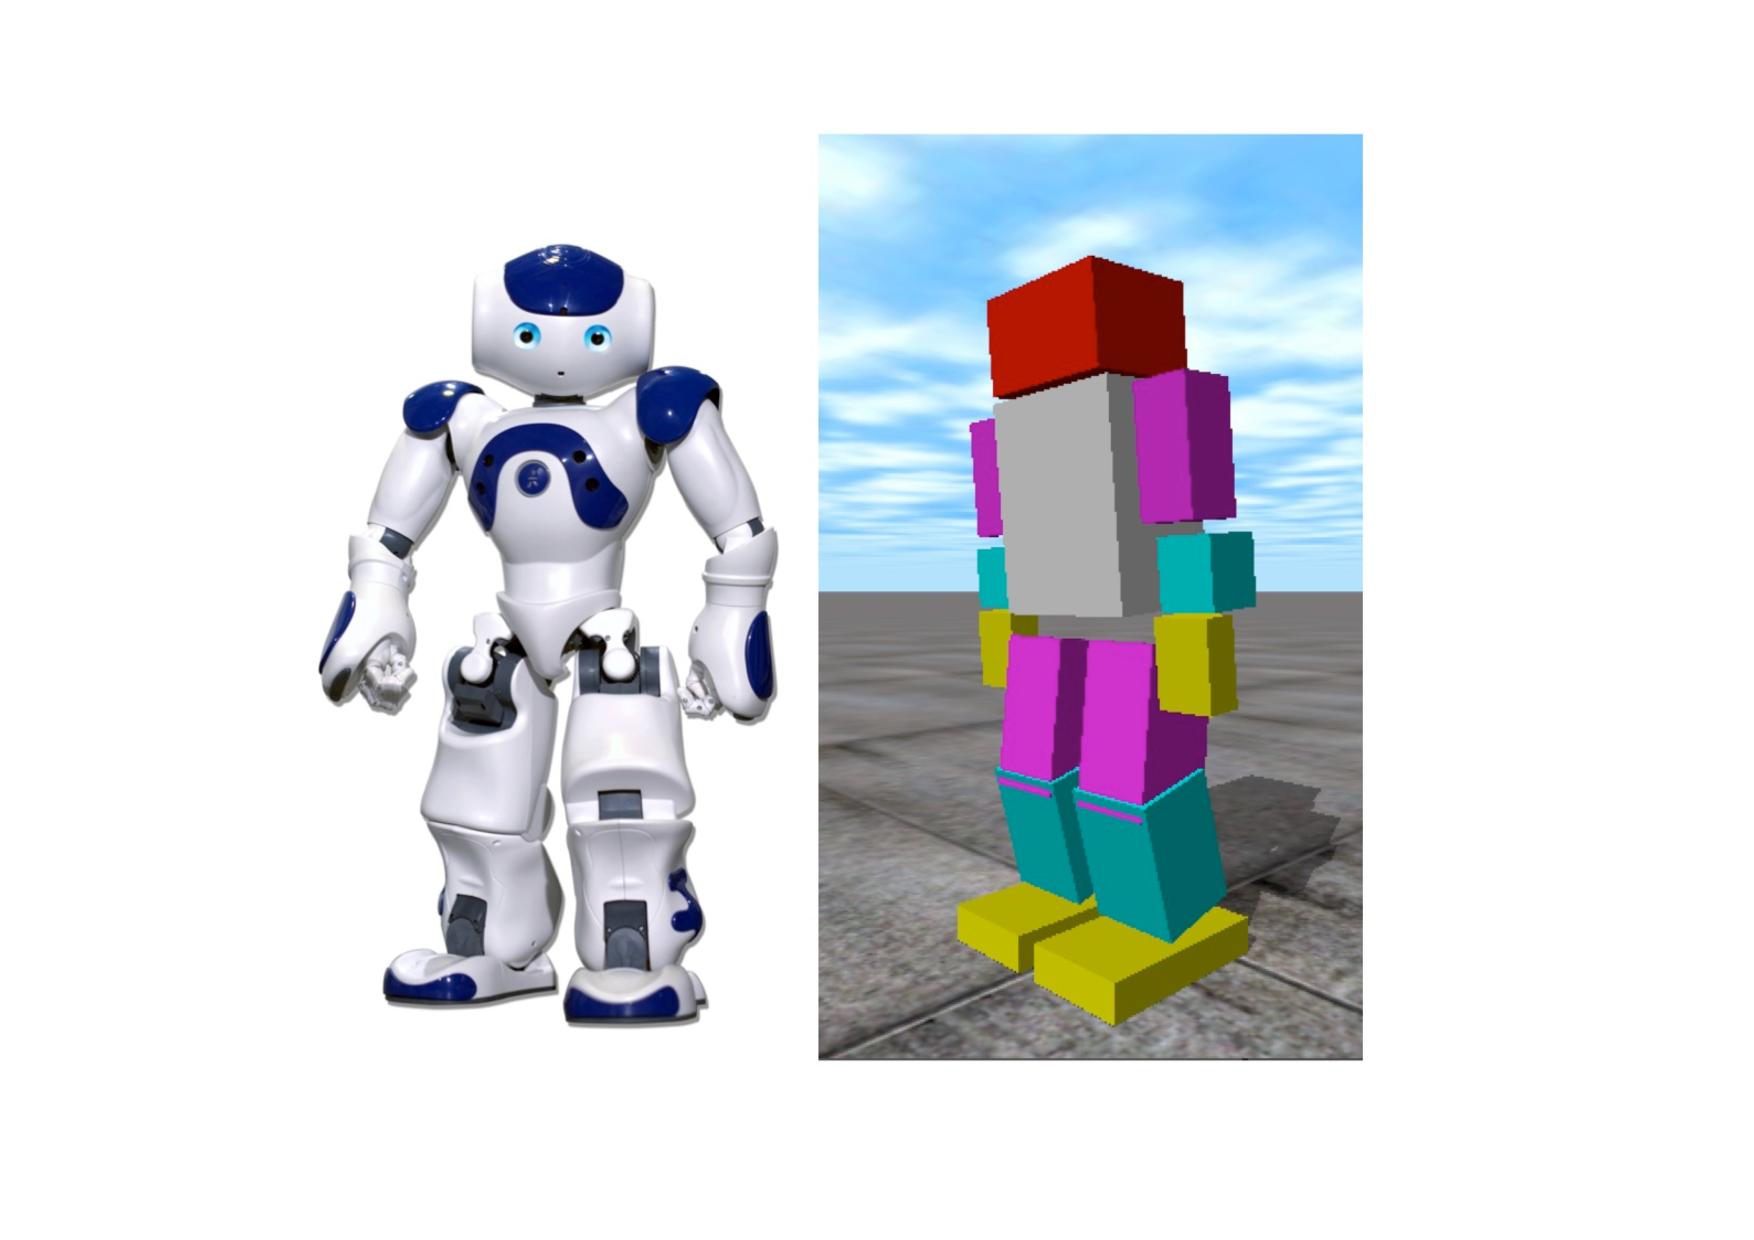
\includegraphics[width=0.42\textwidth]{Figures/NaoSim.pdf}
\caption{Nao Robot and Simulated Version. The box-like rendition of the ODE simulated Nao has been programmed with the precise dimensions, masses, and joint-locations from the manufacturer's specification.} \label{figNao}
\end{figure}

We have used reinforcement learning to learn a policy to stabilise a flat-footed humanoid robot using a physics simulator. The learned policy is supported theoretically and interpreted on a real robot as a linearised continuous control function \cite{hengst2015reinforcement}.  

An interpreter between the behaviour module and the walk engine was introduced in 2015. High level behaviour requests such as lining up to the ball and dribbling are broken down by the interpreter into multiple walk parameters for the walk engine. The interpreter is placed just before the walk engine. Given the state of the walk cycle and the relative ball position, the interpreter ensures precision of steps and a fluid transition between walking and kicking.

Dynamic step size adjustment was improved in 2015. A superellipsoid with axes that represented the maximum forward, side and rotational step was used as a model to constrain directional walk parameters within smooth boundaries.

\section{Odometry}
A visual odometry module was developed in 2012 that estimated the true change in robot's heading by monitoring changes in pixels between vision frames. This is important during external disturbances such as collision with another robot. 

In 2015, z-axis gyroscope measurement was added to Nao H25, which reliably replaced the visual odometry module. The change in heading reported by the walk engine is subsituted with z-axis gyroscope measurement. To avoid drift that occurs when integrating biased gyroscope measurement, walk odometry heading is only replaced when the rates are sufficiently different. The resulting odometry is more accurate and robust to external disturbances.

\section{Path Planning}
Path planning and obstacle avoidance was improved in 2015 by utilising a potential-field based approach, similar to \cite{potentialfields}. The idea is that the robot is moved by the vector sums of the attractive force of the target position and repulsive forces from the obstacles. This is achieved by defining potential functions where the obstacles are on "high ground" and the target is at "low ground". The robot follows the negative gradient of the total potential to get to the target. The method uses little computation and is highly effective.

\section{Goal Detection}

As part of the 2015 rule change, goalposts were converted from yellow to white. This change in colour caused the goalposts to change from being a unique color on the field to becoming the second most common colour, behind only green. The rUNSWift localisation architecture is highly sensitive to false positives, so it was imperative that goal detection for white goals minimised false positive detection. It was also important to still maintain a high detection rate though, so that the robot could remain localised.

The first step in the White Goal detection algorithm is to find regions that may potentially contain goal posts. We call these regions ``candidate regions''. We identify candidate regions based on an isolated property of the goalposts, which is that regardless of the positioning of the robot relative to a goalpost, the base of the goalpost should always intersect with the field edge. With this in mind, our method for generating candidate regions is to scan along the edge of the field and mark pixels identified as white as starting points for candidate regions. Figure \ref{fig:saliencygoal} shows an example goal intersecting the field edge.

\begin{figure}[!ht]
\centering
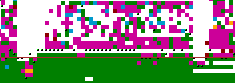
\includegraphics[scale=1.5]{Figures/saliencygoal}
\caption{The detected field edge is shown as a red line}
\label{fig:saliencygoal}
\end{figure}

For each potential starting point, a rectangular region is bound downwards and towards the right whilst the region remains white. This rectangular bound ideally corresponds to the whole base of the goalpost, starting from the field edge to its base.

The candidate region generator uses every white point along the field edge as a starting point to generate rectangular regions. As a result, we are required to cull our candidates such that only the most appropriate regions are left. As such, any candidate region that contains another candidate region, but does not extend further downwards or further outwards(towards the right) are culled from the candidate list. We are then left with the longest candidate regions in each section. An example is provided in Figures \ref{fig:precull} and \ref{fig:postcull}.
\begin{figure}[!ht]
%\begin{floatrow}
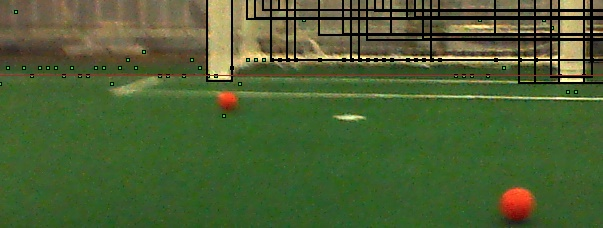
\includegraphics[scale=0.6]{Figures/precull}
\caption{Candidate regions before selective culling}\label{fig:precull}
\end{figure}
\begin{figure}
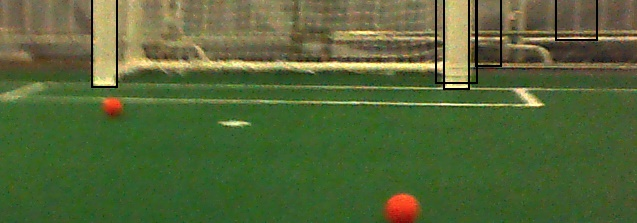
\includegraphics[scale=0.6]{Figures/postcull}
\caption{Candidate regions after selective culling}\label{fig:postcull}
%\end{floatrow}
\end{figure}

The generated candidate regions are extended upwards to cover the entirety of the goalpost above the field edge. This is done through prior knowledge of the goal dimensions, in particular the ratio between the width and height of the goal post. As areas on the field are less prone to noise from background, we are able to reliably determine the width of a goalpost based on the amount of obstruction it imposes on the field edge. This width is then multiplied by 9(the ratio between the height and width of a goalpost) to find the estimated position of the top of the goalpost. The final region is checked against a series of ``sanity checks'', such as the ratio of colour within the region, to ensure that it meets the criteria for being labelled a goal post.

The effectiveness of the 2015 White Goal Detection was measured through lab testing of placing a Nao at particular points on the field and performing a 360$^{\circ}$  rotation. The total number of frames for which a goalpost was correctly classified and incorrectly classified were recorded with a 94\% True Positive rate and a 0.4\% false positive rate. These results are shown in Figures \ref{fig:testpos} and \ref{fig:distaccuracy}.

\begin{figure}[!ht]
%\begin{floatrow}
%\ffigbox{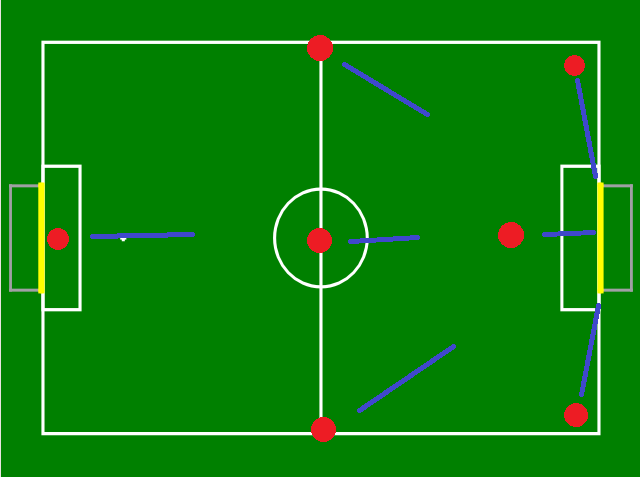
\includegraphics[scale=0.25]{Figures/testpos}}
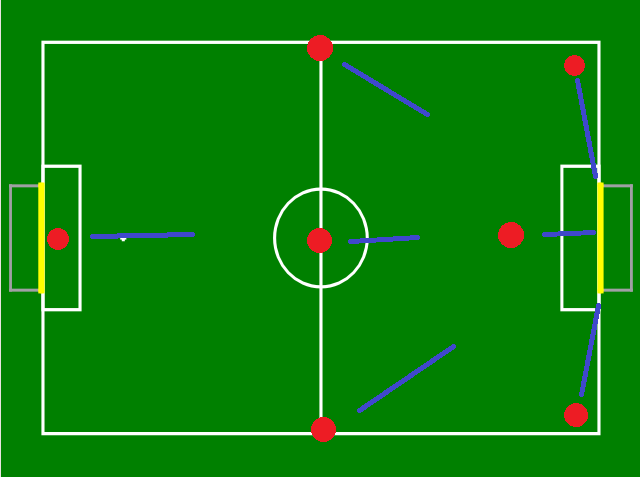
\includegraphics[scale=0.3]{Figures/testpos}
\caption{Goal detection test reference positions}\label{fig:testpos}
\end{figure}
\begin{figure} [h]
%\ffigbox{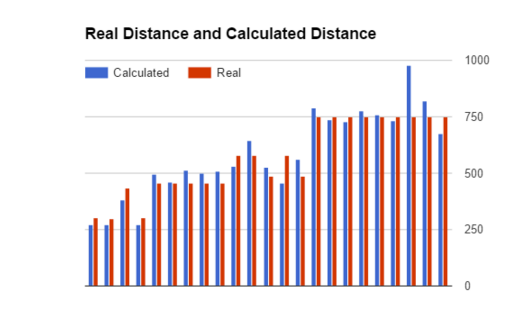
\includegraphics[scale=0.4]{Figures/distaccuracy}}
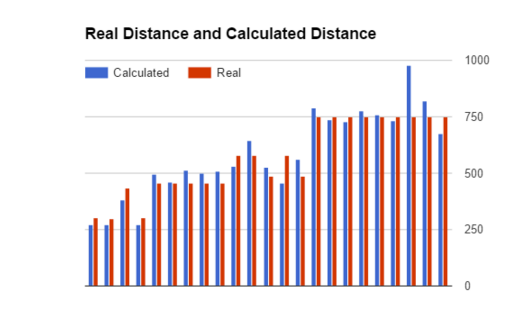
\includegraphics[scale=0.7]{Figures/distaccuracy}
\caption{Calculated distance accuracy}\label{fig:distaccuracy}
%\end{floatrow}
\end{figure}


\section{Concluding Discussion}

After the competition the team members made a list of future developments to overcome weaknesses and add new functionality as a starting point for next year's team. The primary feature identified as needing a big overhaul was the vision system. It is very reliant on accurate colour classification, which can be difficult to achieve with unregulated lighting conditions. The SPL is continuing to move away from distinct colours and regulating the lighting on the field, so we need to make our systems more robust. Our team play is also heavily dependant on reliable wifi connections, which are often not reliable at the competition. This was highlighted by our multiple own goals during the early pool stages when delayed or non-existent wifi packets caused problems for our localisation.

The 2015 team started with a championship quality code base, but also faced a large number of challenges in maintaining and improving the system. With a high student turnover, and many other teams tailoring their strategies to defeat the defending champions, the task of winning back-to-back championships is always challenging. The continued success of team UNSW Australia cannot be attributed to a single factor, or to a single year, but to a combination of integrated software development and team collaboration over several years. 

%The 2014 code and accompanying wiki has been released: \url{https://github.com/UNSWComputing/rUNSWift-2014-release}.

\section*{Acknowledgements}
The 2015 team wish to acknowledge the legacy left by previous rUNSWift teams and the considerable financial and administrative support from the School of Computer Science and Engineering, University of New South Wales. We wish to pay tribute to other SPL teams that inspired our innovations in the spirit of friendly competition, especially to Thomas Hamboeck and the Austrian Kangaroos for their insights into whistle detection methods.





\newpage

\noindent References identified as UNSW CSE Robocup reports and other Robocup related references in this paper are available in chronological order from:

\noindent  \url{ http://cgi.cse.unsw.edu.au/~robocup/2014ChampionTeamPaperReports/ }

\bibliographystyle{splncs03}
\bibliography{SPL2015ChampionTeam}

\end{document}
